%二次方程式の判別式のついて
\documentclass{jsarticle}
\usepackage[dvipdfmx]{graphics}
\usepackage{amsmath}
\usepackage{amssymb}
\usepackage{cases}
\usepackage{docmute}
\usepackage{url}

% \topmargin -0.8in
% \textheight 10in


\title{二次方程式の判別式について}
\author{}
\date{}

\begin{document}
  \maketitle
  \section{二次関数のグラフと二次方程式の解}
  \subsection{グラフの交点の意味}
  グラフの交点の意味を探るべく以下の簡単な二元一次方程式の解を考えたい。
  \begin{numcases}
    {}
    y=2x-1\\
    y=-x+5
  \end{numcases}
  解は容易に解くことができ$x=2$、$y=3$である。\\

  さてここで問題にしたいのはグラフの交点と解の関係である。

  \begin{figure}[htbp]
    \begin{center}
      \resizebox{!}{7cm}{
      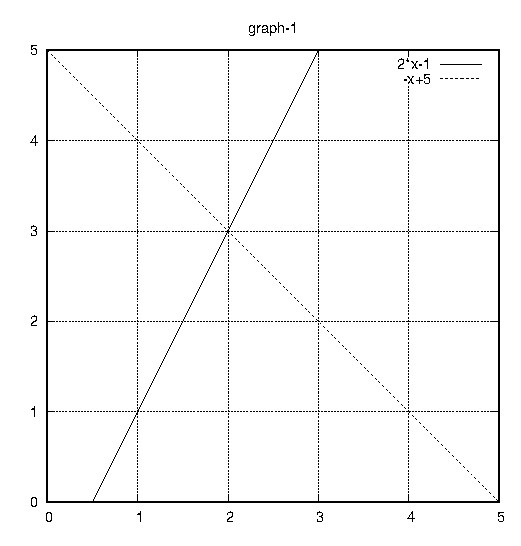
\includegraphics{graph-1-1.eps}
      }
    \end{center}
    \caption{連立方程式とグラフの解の関係}
    \label{fig:graph-1}
  \end{figure}
  式(1)のグラフと式(2)のグラフ交点もやはり$x=2$、$y=3$である。つまり連立方程式の解とはグラフの交点といえる。
  \subsection{二次関数と連立方程式}
  二次関数$x^2-5x+6=0$を以下の連立方程式ととらえることはできないだろうか。
  \begin{numcases}
    {}
    y=x^2-5x+6\\
    y=0
  \end{numcases}
  すると二次方程式の解は、(3)のグラフと$y=0$すなわちx軸との交点であるとわかる。

  \section{二次方程式の実数解の存在}
  \subsection{図形的な解法}
  これまでの内容で、二次方程式の実数解はその二次方程式のグラフして書いたとき、x軸の交点があるかどうかを確認すればよいことがわかる。つまり、放物線の凸の向きと頂点のy座標の2つで答えを出すことができる。

  しかし、これは頂点を求めるための平方完成や、$x^2$の係数からの判断など面倒でかつ間違いやすい。よってここでは新たに{\bf 判別式}という式を導入し簡単に二次方程式の解の個数を決定しよう。

  \subsection{判別式}
  二次方程式$ax^2+bx+c=0$(ただし$a \neq 0$)の判別式を$D$おくと
  \begin{equation}
    D=b^2-4ac
    \label{eq:equation of D}
  \end{equation}
  である。そして以下のことが成立する。
  \begin{enumerate}
    \renewcommand{\labelenumi}{\Roman{enumi}}
    \item $D>0$ならば$ax^2+bx+c=0$の実数解は2つ存在する。
    \item $D=0$ならば$ax^2+bx+c=0$の実数解は1つ存在する。
    \item $D<0$ならば$ax^2+bx+c=0$の実数解は存在しない。
  \end{enumerate}
  ここで二次方程式の解のことを{\bf 実数解}としたが、これは今まで計算で求めてきた解のことを指すので詳しくは述べない。

  \section{判別式の意味}
  判別式は二次方程式の係数から導き出される式であるが、いったいどのような意味なのか二次方程式の解の公式から説明する。まず、$ax^2+bx+c=0$に実数解があるとしてそれを解の公式を用いて求める。そしてそのあとにその解が実数として存在するのかを確認する。
  \subsection{解の公式の吟味}
  $ax^2+bx+c=0$の解の公式は以下の通り
  \begin{equation}
    x=\frac{-b \pm \sqrt{b^2 -4ac}}{2a}
    \label{eq:equation of second degree}
  \end{equation}
  ここで解の公式に注目すると根号の中に判別式と同じ$b^2 -4ac$を見ることができる。なので解の公式に$D$を代入すると
  \begin{equation}
    x=\frac{-b \pm \sqrt{D}}{2a}
    \label{eq:equation of second degree-D}
  \end{equation}
  このように判別式とは、二次方程式の解の公式の根号の中身を表しているものだとわかる。$D$について場合分けをして判別式の意味を考える。
  \begin{enumerate}
    \renewcommand{\labelenumi}{\Roman{enumi}}
    \item $D>0$のとき\\
    この時$\sqrt{b^2-4ac}$は正の値をとる。また解の公式を見直すとその根号の直前に$\pm$がある。つまり$x$には正の数を足したもの、引いたものの二種類があるしたがって実数解が2つあるということである。
    \item $D=0$のとき\\
    この時$\sqrt{b^2-4ac}$は0である。したがって解は$\frac{-b}{2a}$ただ1つである。
    \item $D<0$のとき\\
    この時$\sqrt{b^2-4ac}$は一体どのような値をとるのか。そもそも$\sqrt{a}$は二乗して$a$になる数のことである。しかし$D<0$とはつまり根号の中身が負である。いかなる実数も二乗したら0または正になるためこのような実数$\sqrt{b^2-4ac}$は存在しない。

    $ax^2+bx+c=0$には解があるつもりで解の公式を使ったが、実は解がないことが分かった。
  \end{enumerate}
  \subsection{根号に中身が負である数}
  根号の中身が負である数とは結論から言うと{\bf 虚数}である。今まで整数や分数、小数など様々な数の分類を学んだはずだが、この虚数はその数の種類の1つであると考えてくれたらよい。また、途中から使うようになった{\bf 実数}とはこの虚数という数のグループと対をなすものである。ここでの本題は二次方程式の判別式であるためより詳しい話は別の授業で行う。

\newpage
\documentclass[dvipdfmx]{jsarticle}
\usepackage{graphics}
\usepackage{amsmath}
\usepackage{amssymb}
\usepackage{amsthm}
\usepackage{mathtools}
\usepackage{ascmac}
\usepackage{bm}
\usepackage{url}
\usepackage{txfonts}
\usepackage{color}
\usepackage{tikz}
% \usepackage{docmute}    %パッケージのダウンロードが必要
\usepackage{tikz}
\usetikzlibrary{calc}
\usetikzlibrary{intersections}

\begin{document}
    \section*{最後に}
    本資料は以下のURLのサイトに掲載されているものです.

    {\centering \url{https://blkdenden.firebaseapp.com/lib.html}\\}

    転載などはしないでください.

    また,誤植などは順次訂正しますが,不明な点は掲載サイトのコンタクト欄からメールを送信,または以下のメールアドレスに問い合わせてください.

    {\centering \url{s.kondo11235813@gmail.com}\\}

    % \section*{参考文献}
    % \begin{itemize}
    %     \item 『高等学校 数学B』,数研出版(2017)
    % \end{itemize}




\end{document}


\end{document}
